\documentclass{article}

\usepackage[italian]{babel}
\usepackage[margin=2cm, footskip=5mm]{geometry}
% questi package non sono necessari in lualatex; ref https://tex.stackexchange.com/a/413046
% \usepackage[utf8]{inputenc}
% \usepackage[T1]{fontenc}
\usepackage{enumitem}
\usepackage{hyperref}
\usepackage{titlesec}
\usepackage{soulutf8}
\usepackage{contour}
\usepackage{float}
\usepackage{graphicx}
\usepackage{fancyhdr}
\usepackage{longtable}
\usepackage[table]{xcolor}
\usepackage{titling}
\usepackage{lastpage}
\usepackage{ifthen}
\usepackage{calc}
\usepackage{minted}
\usepackage{pgfgantt}
\usepackage{subfiles}

\newlength{\imgwidth}

\newcommand\scalegraphics[1]{%
    \settowidth{\imgwidth}{\includegraphics{#1}}%
    \setlength{\imgwidth}{\minof{\imgwidth}{\textwidth}}%
    \includegraphics[width=\imgwidth]{#1}%
}

% XXX definizione dei percorsi in cui cercare immagini
\graphicspath{ {./}
    {./img/}
}

% esempio di utilizzo: \appendToGraphicspath{./img/} (un comando diverso per ogni path da includere)
% N.B.: ci DEVE essere un forward slash alla fine del path, a indicare che è una cartella.
\makeatletter
\newcommand\appendToGraphicspath[1]{%
  \g@addto@macro\Ginput@path{{#1}}%
}
\makeatother

% setup della sottolineatura
\setuldepth{Flat}
\contourlength{0.8pt}

\newcommand{\uline}[1]{%
  \ul{{\phantom{#1}}}%
  \llap{\contour{white}{#1}}%
}

% setup dei link
\hypersetup{
  colorlinks=true, % set true if you want colored links
  linktoc=all,     % set to all if you want both sections and subsections linked
  linkcolor=black, % choose some color if you want links to stand out
}

% setup di header e footer
\pagestyle{fancy}

\fancyhf{}
\fancyhead[L]{\includegraphics[width=1cm]{logo.png}}
\fancyhead[R]{\thetitle}
\fancyfoot[R]{\thepage\ di~\pageref{LastPage}}

\fancypagestyle{nopage}{%
  \fancyfoot{}%
}

\setlength{\headheight}{1.2cm}

% setup forma \paragraph e \subparagraph
\titleformat{\paragraph}[hang]{\normalfont\normalsize\bfseries}{\theparagraph}{1em}{}
\titleformat{\subparagraph}[hang]{\normalfont\normalsize\bfseries}{\thesubparagraph}{1em}{}

% setup profondità indice di default
\setcounter{secnumdepth}{5}
\setcounter{tocdepth}{5}

% shortcut per i placeholder
\newcommand{\plchold}[1]{\textit{\{#1\}}} % chktex 20

% hook per lo script che genera il glossario
\newcommand{\glossario}[1]{\underline{#1}\textsubscript{g}}

% definizione dei comandi \uso e \stato
\makeatletter
\newcommand{\setUso}[1]{%
  \newcommand{\@uso}{#1}%
}
\newcommand{\uso}{\@uso}

\newcommand{\setStato}[1]{%
  \newcommand{\@stato}{#1}%
}
\newcommand{\stato}{\@stato}

\newcommand{\setVersione}[1]{%
  \newcommand{\@versione}{#1}%
}
\newcommand{\versione}{\@versione}

\newcommand{\setResponsabile}[1]{%
  \newcommand{\@responsabile}{#1}%
}
\newcommand{\responsabile}{\@responsabile}

\newcommand{\setRedattori}[1]{%
  \newcommand{\@redattori}{#1}%
}
\newcommand{\redattori}{\@redattori}

\newcommand{\setVerificatori}[1]{%
  \newcommand{\@verificatori}{#1}%
}
\newcommand{\verificatori}{\@verificatori}

\newcommand{\setDescrizione}[1]{%
  \newcommand{\@descrizione}{#1}%
}
\newcommand{\descrizione}{\@descrizione}

\newcommand{\setModifiche}[1]{%
  \newcommand{\@modifiche}{#1}%
}

\newcommand{\modifiche}{\@modifiche}

\makeatother

% setup delle description
\setlist[description,1]{font=$\bullet$\hspace{1.5mm}, labelwidth=* leftmargin=*,labelindent=12.5mm}
\setlist[description,2]{font=$\bullet$\hspace{1.5mm}, leftmargin=*,labelindent=12.5mm}
\appendToGraphicspath{../../commons/img/}

\title{Verbale interno --- 05/03/2020}

\setResponsabile{Riccardo Agatea}
\setRedattori{Alberto Gobbo}
\setVerificatori{
  Tobia Apolloni
}
\setUso{Interno}
\setDescrizione{Verbale dell'incontro di GruppOne del 05/03/2020}
\setModifiche{%
\cellcolor{white!80!lightgray!100} & Riccardo Agatea & 2020--03--07 & approva documento \\%
\cellcolor{white!80!lightgray!100} & Verificatore & 2020--03--06 & verifica verbale \\%
\multirow{-3}{*}{-} \cellcolor{white!80!lightgray!100} & Alberto Gobbo & 2020--03--05 & stendi verbale %
}

\disabilitaVersione{}
\disabilitaElencoFigure{}
\disabilitaElencoTabelle{}

\begin{document}

\thispagestyle{empty}
\pagenumbering{gobble}

\begin{center}

  \includegraphics[width=8.5cm]{\commons/img/logo.png}\\
  {\Large GruppOne - progetto "Stalker"}\\
  \vspace{1.5cm}

  {\Huge \thetitle}
  \vspace{1.5cm}

  \begin{table}[H]
    \centering

    \begin{tabular}{r|l}
      \textbf{Versione}     & \versione              \\
      \textbf{Approvazione} & \responsabile          \\
      \textbf{Redazione}    & \redattori             \\
      \textbf{Verifica}     & \verificatori          \\
      \textbf{Stato}        & \stato                 \\
      \textbf{Uso}          & \uso                   \\
      \textbf{Destinato a}  & Imola Informatica      \\
                            & GruppOne               \\
                            & Prof. Tullio Vardanega \\
                            & Prof. Riccardo Cardin  \\
    \end{tabular}
  \end{table}

  \vspace{3cm}
  \textbf{Descrizione}\\
  \descrizione\\
  \vfill
  \verb|gruppone.swe@gmail.com|
\end{center}

\newpage
\thispagestyle{nopage}

\section*{Registro delle modifiche}
\label{sec:registro_delle_modifiche}

\begin{table}[H]
  \label{tab:registro_delle_modifiche}

  \centering
  \rowcolors{2}{lightgray}{white!80!lightgray!100}

  \begin{longtable}[c]{c c c c l}
    \rowcolor{darkgray!90!}\color{white}{\textbf{Versione}} & \color{white}{\textbf{Data}} & \color{white}{\textbf{Nominativo}} & \color{white}{\textbf{Ruolo}} & \color{white}{\textbf{Descrizione}} \\\endhead
    \modifiche
  \end{longtable}
\end{table}

% section registro_delle_modifiche (end)
\newpage

\thispagestyle{nopage}
\pagenumbering{roman}
\tableofcontents

\newpage

\pagenumbering{arabic}


\section{Informazioni logistiche}%
\label{sec:informazioni_logistiche}

\begin{description}
  \item [Luogo] chiamata Hangouts
  \item [Data] 05/03/2020
  \item [Ora] 15:30 \symbol{8594} 17:30
\end{description}

\subsection{Membri del gruppo presenti}%
\label{sub:membri_del_gruppo_presenti}

\begin{enumerate}
  \item Riccardo Agatea
  % \item Tobia Apolloni
  \item Riccardo Cestaro
  \item Alberto Cocco
  \item Luca Ercole
  \item Alberto Gobbo
  \item Alessandro Rizzo
  \item Fabio Scettro
\end{enumerate}
% sub:membri_del_gruppo_presenti (end)
% sec:informazioni_logistiche (end)

\section{Introduzione}%
\label{sec:introduzione}

Abbiamo definito lo schema relazionale del database che verrà sviluppato in MySQL che sarà fondamentale per tutte le interrogazioni che saranno effettuate dal back-end e front-end del sistema di Stalker.

Inoltre abbiamo preso decisioni che erano rimaste in sospeso dall'ultimo incontro, in merito all'ambiente di sviluppo da utilizzare per il front-end e agli strumenti per lo sviluppo del layout grafico di applicazione mobile e web application.

\section{Ordine del giorno}%
\label{sec:ordine_del_giorno}

\begin{itemize}
  \item Definizione struttura schema relazionale per il database MySQL\@.
  \item Decisioni finali su tecnologie da utilizzare.
\end{itemize}
% sec:ordine_del_giorno (end)

\section{Definizione struttura schema relazionale per il database MySQL}%
\label{sec:definizione_struttura_schema_relazionale_per_il_database_MySQL}
Il gruppo ha lavorato congiuntamente per realizzare lo schema relazionale del database MySQL che verrà utilizzato nel sistema di Stalker per memorizzare tutti i dati relativi agli utenti registrati e alle organizzazioni nel loro complesso.

Abbiamo utilizzato GenMyModel (\href{https://www.genmymodel.com/}{https://www.genmymodel.com/}), uno strumento online per costruire diagrammi e molto altro.

L'attività principale svolta è stata l'individuazione di tutte le entità, le relazioni tra esse e gli attributi coinvolti.

Lo schema relazionale sarà ulteriormente raffinato a partire dal documento di \textit{Analisi dei Requisiti} per aggiungere i dettagli mancanti.

Una volta ultimato, lo schema concettuale sarà definito in un database relazionale MySQL che servirà per comunicare i dati d'interesse all'applicazione mobile e alla web application.

% sec:definizione_struttura_schema_relazionale_per_il_database_MySQL (end)

\section{Decisioni finali su tecnologie da utilizzare}%
\label{sec:decisioni_finali}

\subsection{Scelta ambiente di sviluppo per l'applicazione mobile}%
\label{sub:scelta_ambiente_di_sviluppo_per_applicazione_mobile}
Il gruppo ha valutato attentamente quale ambiente di sviluppo utilizzare per lo sviluppo dell'applicazione mobile tra Android Studio e IntelliJ IDEA\@.

Nonostante Android Studio sia un ambiente di sviluppo dedicato alle applicazioni Android, i requisiti di sistema minimi sono troppo onerosi per i computer di alcuni membri del gruppo.

Vista la possibilità di sviluppare applicazioni Android e un ambiente di sviluppo più leggero, la scelta è ricaduta su IntelliJ IDEA 2019.3.3 versione Community, in quanto la licenza è gratuita.
% sub:scelta_ambiente_di_sviluppo_per_applicazione_mobile (end)

\subsection{Scelta strumenti per design applicazione mobile e web application}%
\label{sub:scelta_strumenti_per_design_applicazione_mobile_e_web_application}
Per l'aspetto grafico dell'applicazione mobile, è stato scelto il linguaggio visuale di Google \glossario{Material design}, in quanto c'è un'ampia documentazione per Android che descrive i vari componenti grafici e i temi da applicare all'applicazione.

Per quanto riguarda l'aspetto grafico della web application, è stato scelto \glossario{Bootstrap}, una piattaforma per la creazione di contenuti web che offre un'ampia documentazione.

% sub:scelta_strumenti_per_design_applicazione_mobile_e_web_application (end)

% sec:varie_ed_eventuali (end)

\newpage
\section{Registro delle decisioni}%
\label{sec:registro_delle_decisioni}

\begin{description}
  \item[20200305-int-001] Abbiamo definito lo schema relazionale per definire il database relazionale MySQL del sistema di Stalker.
  \item[20200305-int-002] Abbiamo deciso che l'ambiente di sviluppo da utilizzare per lo sviluppo dell'applicazione mobile sarà IntelliJ IDEA\@.
  \item[20200305-int-003] Abbiamo deciso che per il linguaggio visuale per l'applicazione mobile sarà utilizzato Material Design.
  \item[20200305-int-004] Abbiamo deciso che per la grafica della web application sarà utilizzata la piattaforma web Bootstrap.
\end{description}

% sec:registro_delle_decisioni (end)

\end{document}
